% Slides for the 16 Oct 2026 meeting with Danni and Tianyi (10 minutes).
% Compile: tectonic slides.tex   (from this folder)
% Numbers: docs/NEXT_STEPS.md section 1a (final, 12 Oct). Script:
% Meeting_Prep_Oct16.md part 2. AI assistance: Claude made these slides
% from the project's results; Brian presents them.
\documentclass[aspectratio=169,11pt]{beamer}
\usetheme{default}
\setbeamertemplate{navigation symbols}{}
\setbeamertemplate{footline}[frame number]
\setbeamerfont{frametitle}{size=\large,series=\bfseries}
\usepackage{booktabs}
\graphicspath{{../../paper/figures/}{../../travel-speed-gate1/results/t2_terrain_effects/}{../../travel-speed-gate1/results/t4_terrain_curve/}{../../travel-speed-gate1/results/t4_trail_map/}{../../travel-speed-gate1/results/t4_mode_curves/}}
\definecolor{accent}{HTML}{2A78D6}
\setbeamercolor{frametitle}{fg=accent}
\setbeamercolor{structure}{fg=accent}

\title{Hiking speed from GPS traces and remote sensing}
\subtitle{Status since 9 Oct: T1 complete, T2 tier 1, first T3 results}
\author{Brian Zhou\\\small mentors Danni Beaulieu, Tianyi Gao; advisor Prof.\ Nathan Jacobs}
\date{16 Oct 2026}

\begin{document}

\begin{frame}
\titlepage
\end{frame}

\begin{frame}{Since 9 Oct}
\begin{itemize}\setlength\itemsep{6pt}
\item \textbf{T1 complete: 17 regions} (US and Canada). 16 from full OSM
  downloads plus the lab crawl; the Bay Area from the crawl only.
  \begin{itemize}
  \item 2,876 hiking traces; walking set: 1,992 outings, 4,702 moving hours
  \item 290,640 walking segments of 50 m, one combined dataset and data card
  \end{itemize}
\item \textbf{T2 tier 1 done for all regions}: terrain from 5 m and 1 m
  elevation, 30 m vegetation, AlphaEarth satellite embeddings.
\item \textbf{T3 evaluation harness}: every model predicts a speed
  \emph{range} per segment and is graded only on hikes, map squares or
  \textbf{whole regions} it never saw (CRPS, coverage, hike time).
\item \textbf{Lead result}: terrain from remote sensing transfers to unseen
  regions; map tags barely do.
\end{itemize}
\end{frame}

\begin{frame}{The dataset}
\centering
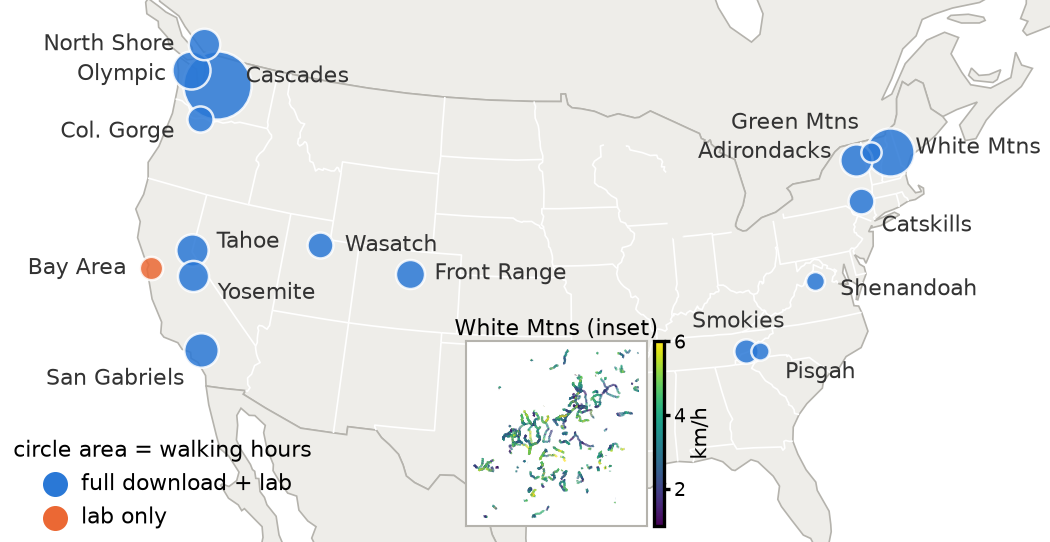
\includegraphics[width=0.78\textwidth]{fig_map}\\[2pt]
\small Circle area = walking hours. Inset: White Mountains segments by speed.
\end{frame}

\begin{frame}{Speed vs slope: Tobler is too fast and too lopsided}
\begin{columns}[c]
\column{0.5\textwidth}
\centering
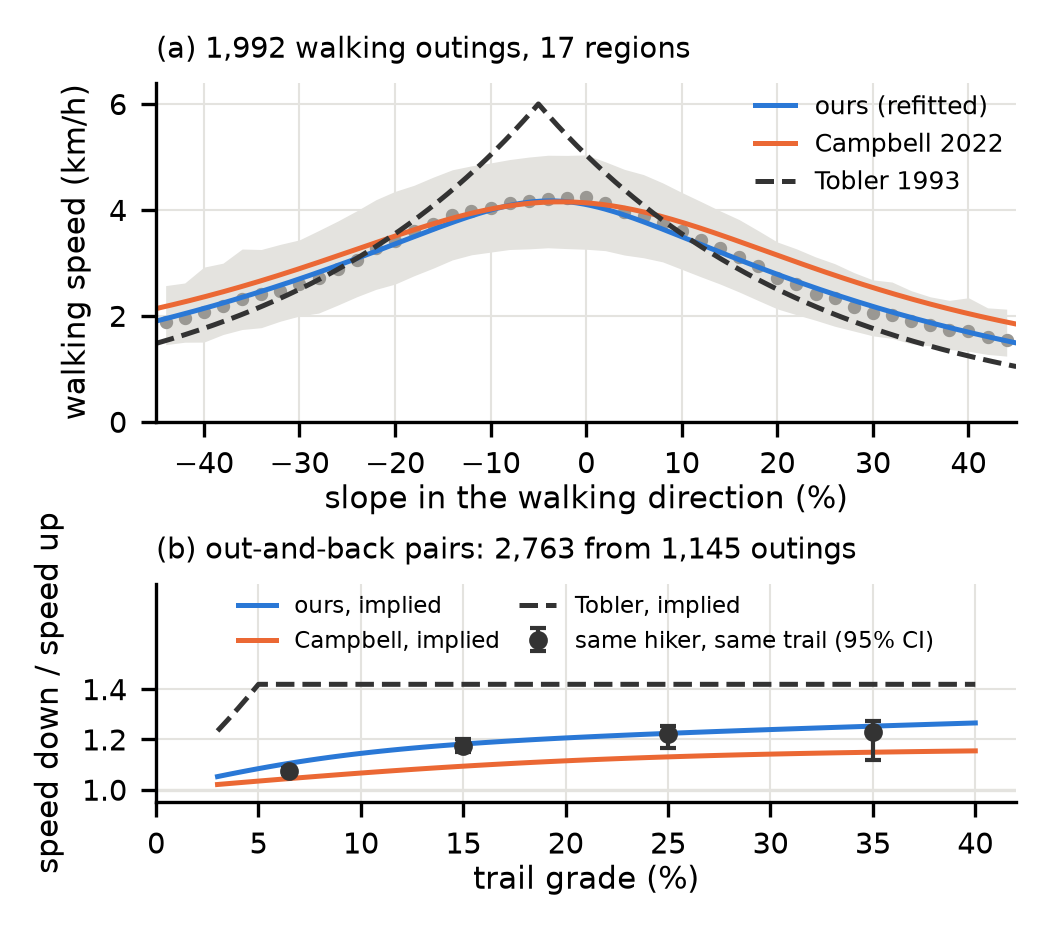
\includegraphics[height=0.84\textheight]{fig_curve}
\column{0.48\textwidth}
\small
\begin{itemize}\setlength\itemsep{5pt}
\item Measured speed peaks near \textbf{4.2 km/h} on level to gently
  descending trail (Tobler: 6.0).
\item Tobler: $\sim$20\% too fast on gentle grades, $\sim$18\% too slow on
  climbs over 25\%.
\item Campbell 2022: right near level, $\sim$20\% too fast on steep climbs.
\item Same hiker, same trail (2,763 out-and-back pairs): downhill is 8\%
  faster than uphill at 3--10\% grade, 22\% above 20\%. Tobler says 42\%
  everywhere.
\end{itemize}
\end{columns}
\end{frame}

\begin{frame}{How we test}
\begin{columns}[T]
\column{0.5\textwidth}
\textbf{Three ways to hide data}
\begin{itemize}
\item new hikers (5 folds of outings)
\item new places (5 folds of 10 km squares)
\item \textbf{a new region} (leave one of 17 out)
\end{itemize}
\textbf{Score}: CRPS skill vs a slope curve refitted to our data; 95\%
intervals resample whole regions.
\column{0.5\textwidth}
\textbf{Models}
\begin{itemize}
\item published: Tobler 1993, Campbell et al.\ 2022, STRIDE 2024
\item slope curve (baseline)
\item + OSM tags / + terrain / + embeddings / + vegetation\\
  (additive model and boosted trees)
\item references: the hiker's own pace (first km), the region's own offset
\end{itemize}
\end{columns}
\end{frame}

\begin{frame}{Lead result: terrain transfers, tags don't}
\begin{columns}[c]
\column{0.5\textwidth}
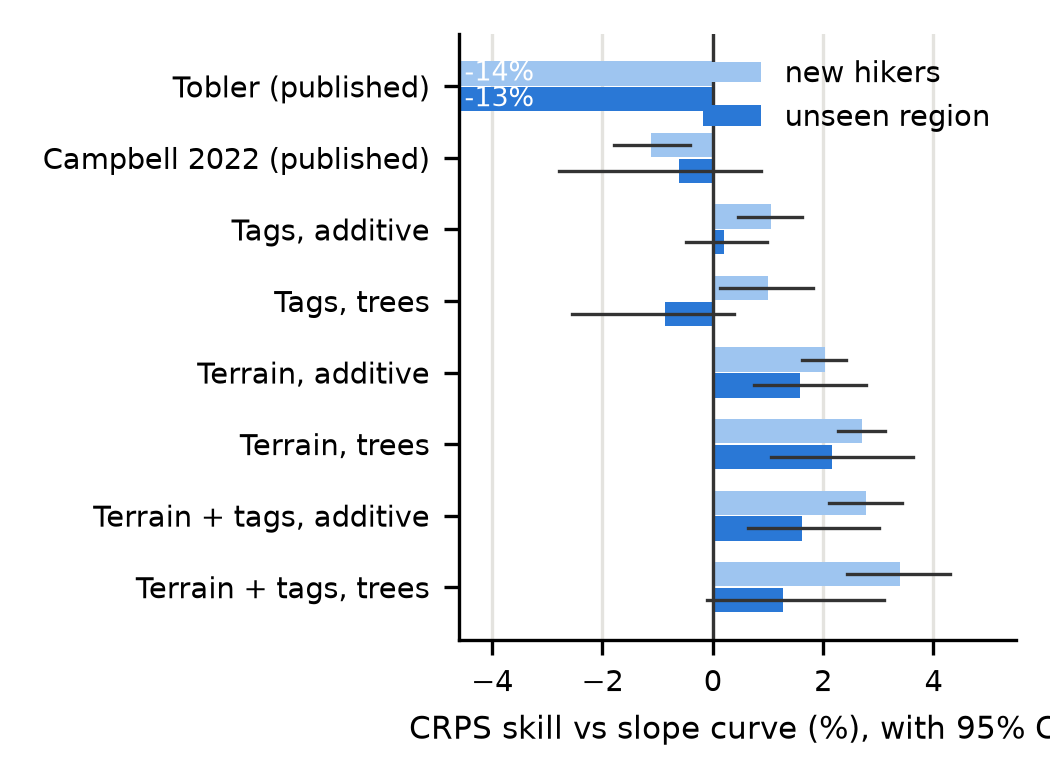
\includegraphics[width=\textwidth]{fig_skill}
\column{0.48\textwidth}
\footnotesize
\begin{tabular}{@{}lr@{}}
\toprule
Unseen region & skill [95\% CI] \\
\midrule
Tobler 1993 & $-12.5\%$ \\
STRIDE 2024 & $-16.8\%$ \\
Campbell 2022 & $-0.5\%$ \\
OSM tags & $+0.9\%$ [0.1, 1.7] \\
Embeddings & $+1.1\%$ [0.1, 2.6] \\
\textbf{Terrain} & $\mathbf{+2.1\%}$ [1.5, 3.1] \\
\textbf{Terrain (trees)} & $\mathbf{+2.8\%}$ [1.8, 4.1] \\
Terrain + emb.\ + tags (trees) & $+3.9\%$ [2.7, 5.7] \\
\bottomrule
\end{tabular}\\[4pt]
Terrain beats tags in \textbf{16 of 17} held-out regions.\\[2pt]
All models get their range the same way: prediction + error spread on
held-out training hikes.
\end{columns}
\end{frame}

\begin{frame}{Per region: terrain beats tags in 16 of 17}
\begin{columns}[c]
\column{0.55\textwidth}
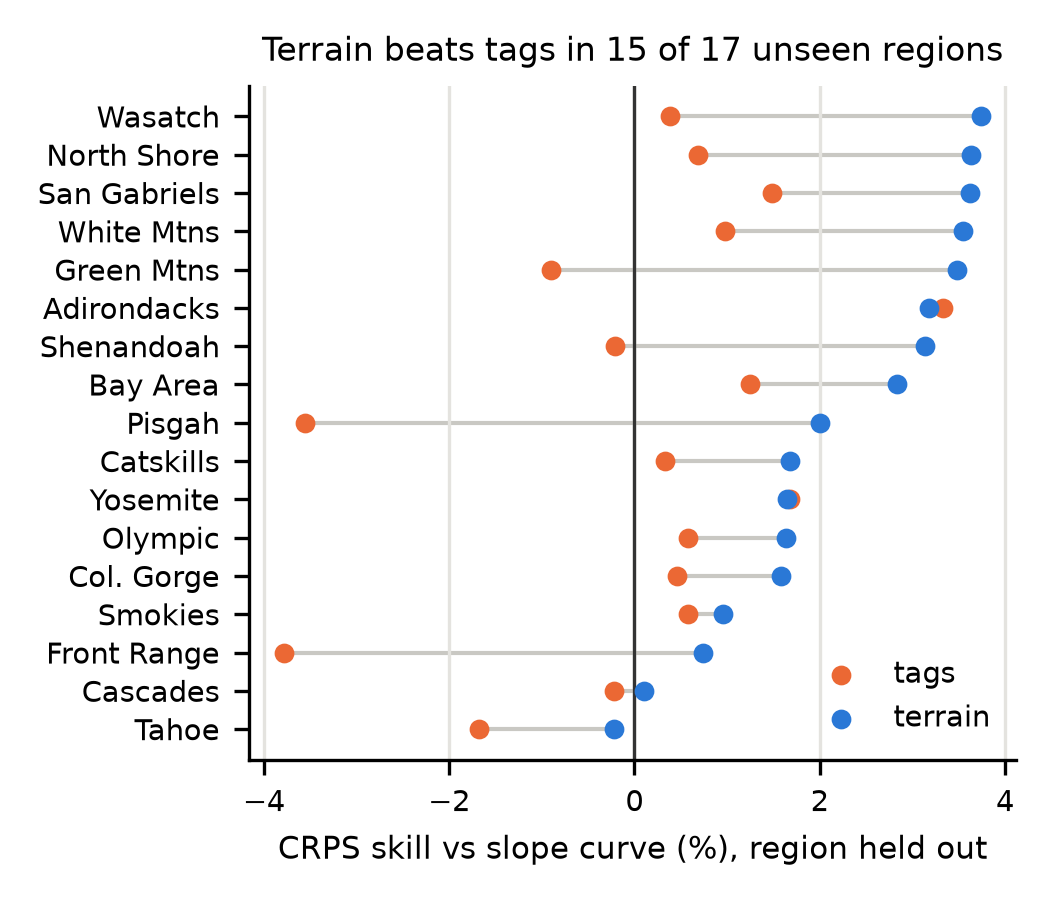
\includegraphics[height=0.8\textheight]{fig_regions}
\column{0.43\textwidth}
\small
\begin{itemize}\setlength\itemsep{4pt}
\item Terrain minus tags: $+0.7$ to $+2.2$ points (95\%), above zero in
  every bootstrap draw.
\item In 5 regions tags make predictions \emph{worse} (Tahoe, Pisgah,
  Shenandoah, Front Range, Green Mtns); terrain helps in all 17.
\item The exception: Yosemite (tags $+1.9$, terrain $+1.1$).
\item Why tags fail: within a hike they act the same everywhere; but
  sac\_scale is on 1--96\% of trail by region, and ``no tag'' means
  different things in different regions.
\end{itemize}
\end{columns}
\end{frame}

\begin{frame}{What ``terrain'' means}
\centering
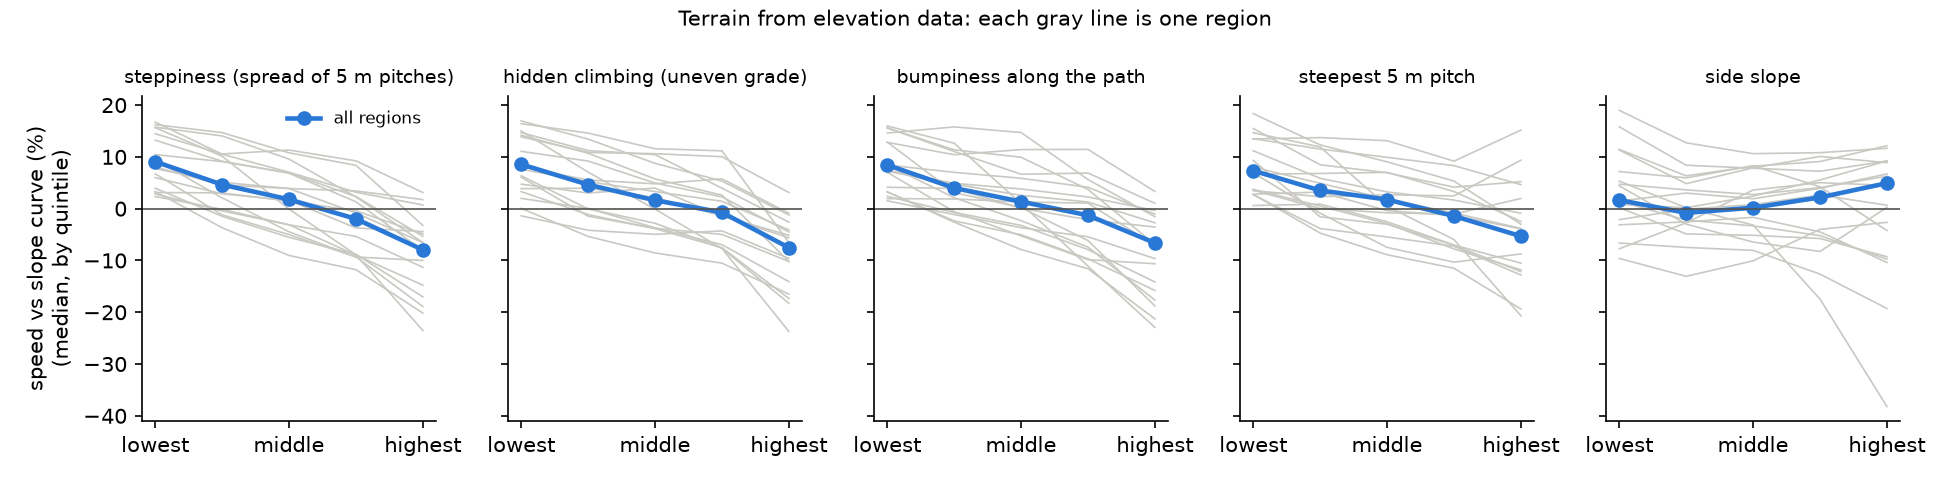
\includegraphics[width=\textwidth]{fig_quintiles}\\[4pt]
\raggedright\small Read every 1 m along the matched path from the elevation
grid. Gray: one line per region; blue: all regions. Steppier trail profiles
are slower everywhere: smoothest fifth $+9\%$, steppiest fifth $-8\%$
vs slope alone. The gain in unseen regions is largest on descents and level
trail ($+2.3$ to $+2.8\%$), smallest on steep climbs ($+0.8\%$): footing
limits descents, effort limits climbs.
\end{frame}

\begin{frame}{Checks}
\small
\begin{itemize}\setlength\itemsep{3pt}
\item \textbf{Not a region proxy}: terrain still adds $\sim$1.9 points over
  each region's own speed offset.
\item \textbf{Not a hiker proxy}: still $\sim$2.3 points once the hiker's
  pace is known.
\item \textbf{No neighbours in training}: a whole zone held out, terrain
  $+1.9\%$ (tags $+0.7\%$); West $\leftrightarrow$ East $+2.6\%$ (tags
  $+1.5\%$). \textbf{Newer hikes} $+2.2\%$. \textbf{Season, time of day,
  weather} add nothing in new regions.
\item \textbf{GPS rate}: the same gain for traces recorded every $\le$2 s,
  2--10 s, $>$10 s ($+1.7$, $+2.4$, $+1.9\%$). Sparse traces read
  $\sim$10\% slow; thinning dense walks reproduces it (cut corners, hidden
  stops).
\item \textbf{Hidden climbing}: $\sim$60\% of the gain is uneven grade inside
  the 50 m segment; the rest is difficulty beyond grade.
\item \textbf{1 m lidar $\approx$ 5 m} for this signal; STRIDE's roughness adds
  nothing on trails.
\item \textbf{30 m vegetation adds nothing}; \textbf{embeddings} help
  within regions ($+2.6\%$) but transfer less reliably ($+1.1\%$).
\item \textbf{Calibration}: 90\% ranges hold 88--90\%; a terrain-dependent spread
  doesn't help.
\item \textbf{Mode labels}: 5\% of ``walkers'' are labeled bike/ski by their
  own app (327 labeled traces).
\end{itemize}
\end{frame}

\begin{frame}{A terrain-adjusted Tobler formula}
\begin{columns}[c]
\column{0.58\textwidth}
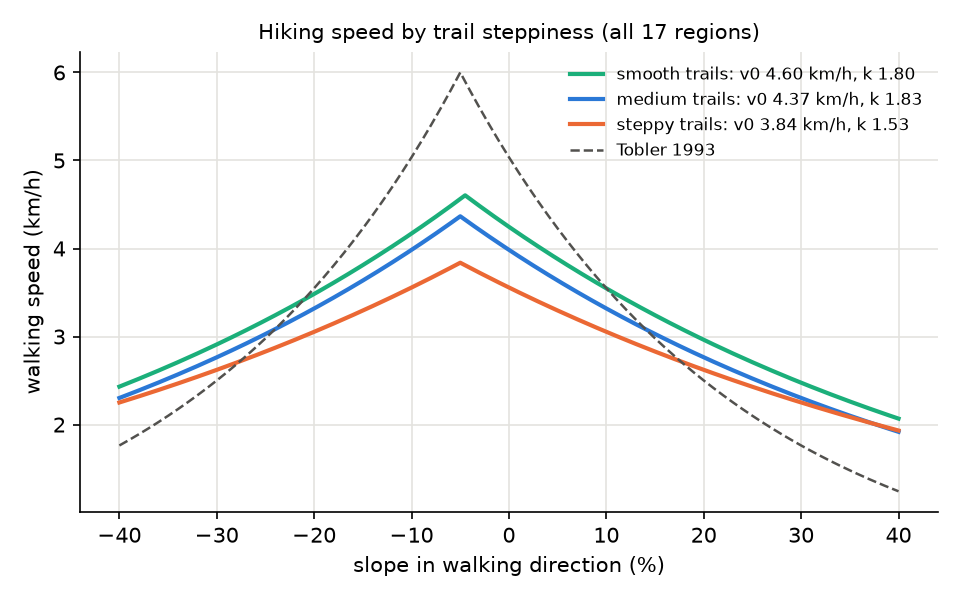
\includegraphics[width=\textwidth]{fig_curves}
\column{0.4\textwidth}
\small
\[\ln v = a_0 + a_1 z - (k_0 + k_1 z)\,|s + s_0|\]
$z$ = spread of 5 m pitches $/\,0.10$ (one number from any DEM).
\begin{itemize}\setlength\itemsep{4pt}
\item Peak: smooth trails 4.60, steppy 3.84 km/h (Tobler: 6.0).
\item $+1.0\%$ [0.6, 1.5] in unseen regions with 5 numbers; less
  portable than the full models ($+0.6\%$ for an unseen zone).
\item A drop-in for GIS tools that use Tobler today.
\end{itemize}
\end{columns}
\end{frame}

\begin{frame}{Pace on every White Mountains trail}
\centering
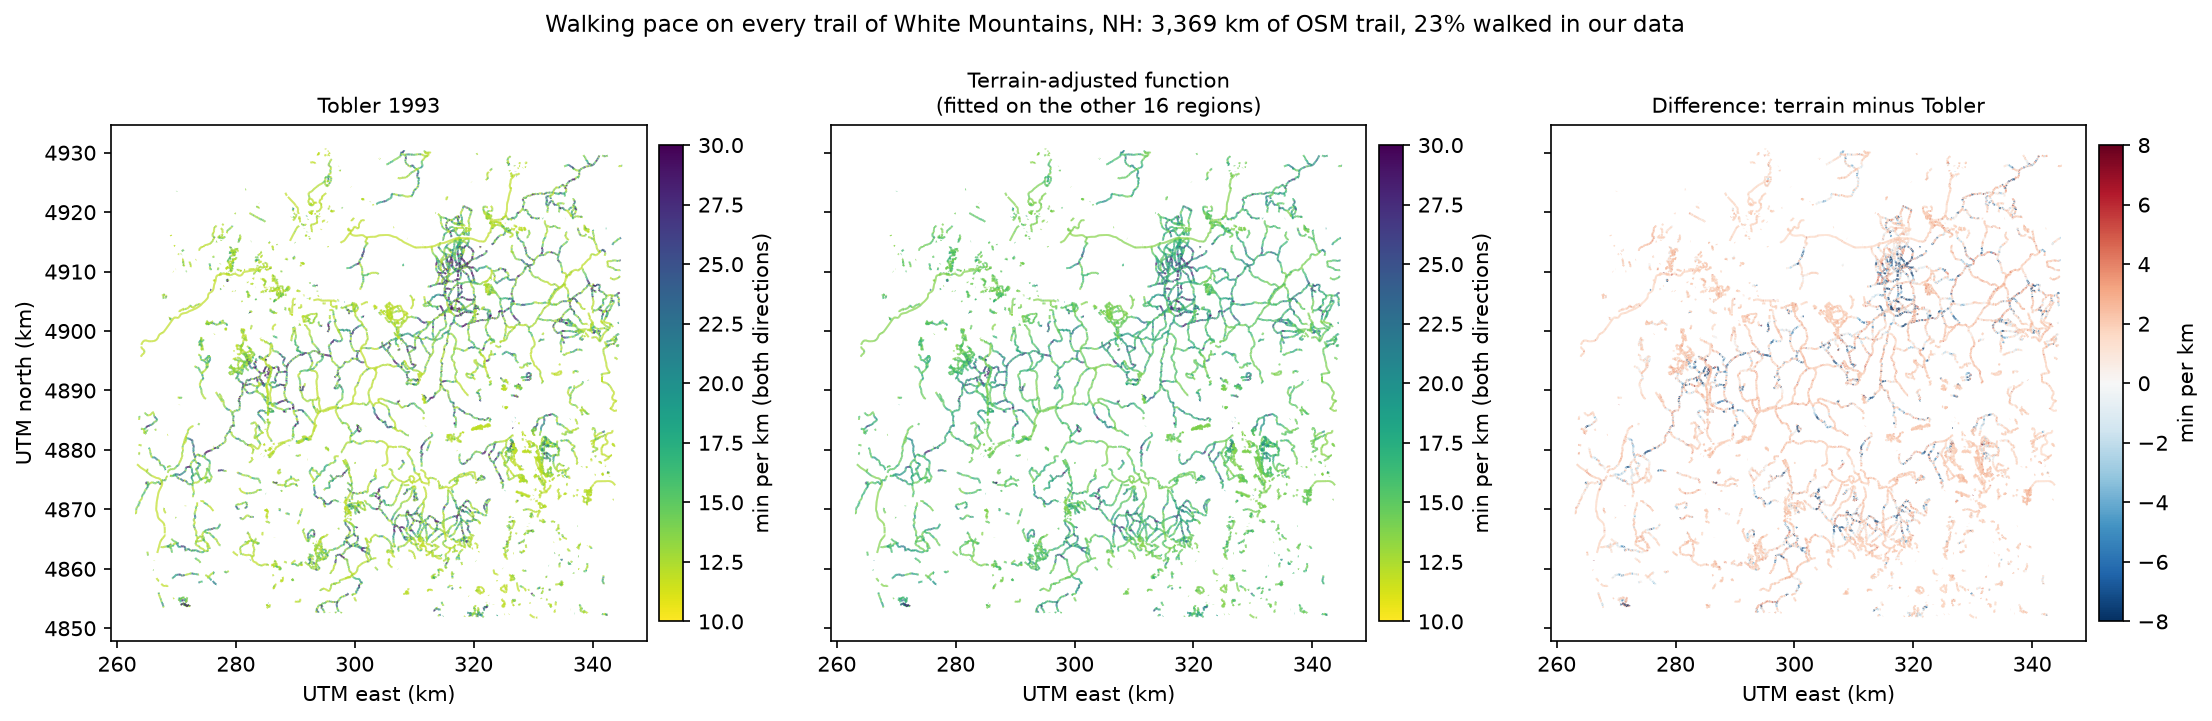
\includegraphics[width=\textwidth]{fig_wm_pace}\\[4pt]
\raggedright\small 3,369 km of OSM trail, 77\% never walked in our data.
The formula is fitted on the other 16 regions. Right: difference from
Tobler.
\end{frame}

\begin{frame}{Travel modes on the same trails}
\centering
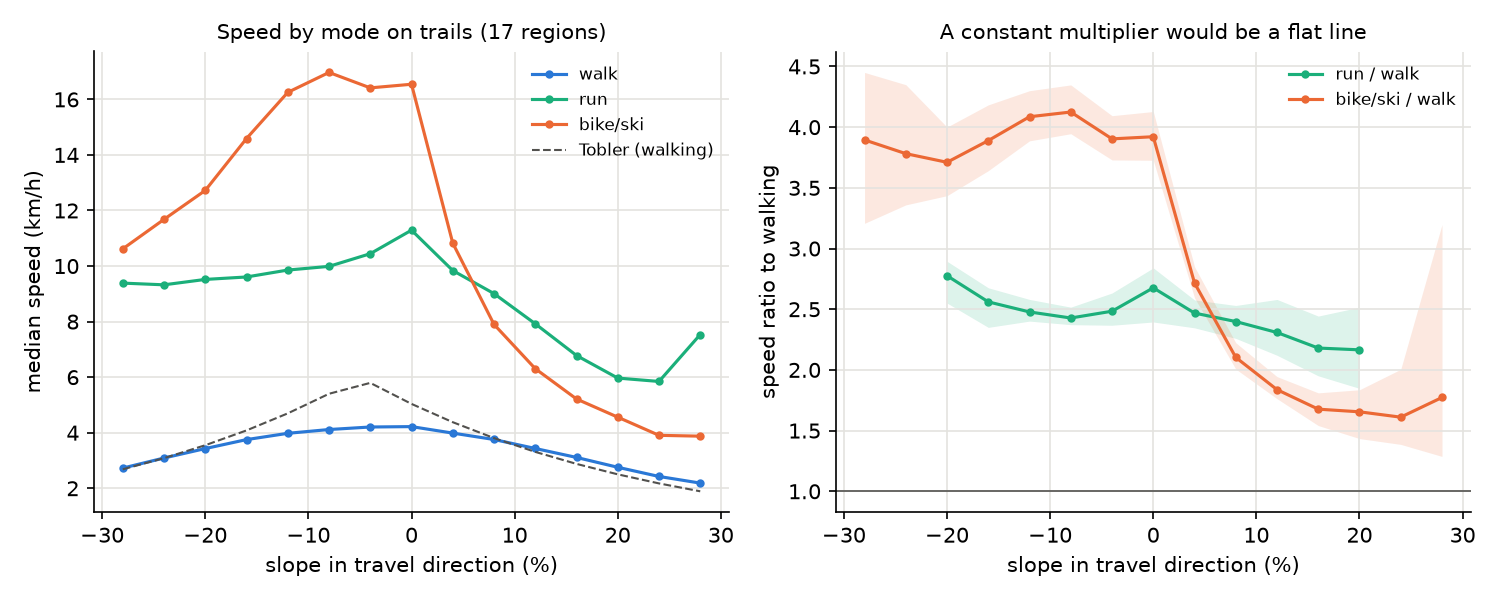
\includegraphics[width=0.92\textwidth]{fig_modes}\\[4pt]
\raggedright\small Bike/ski $\approx 4\times$ walking on descents but
$\approx 1.6\times$ on climbs, so a constant mode multiplier fails.
Runners $\approx 2.5\times$. On held-out hikes, a constant $\times$2.5 is as
good as a runner curve of its own; bikes and skis need their own (3.8\%
better).
\end{frame}

\begin{frame}{Whole hikes: the hiker matters most}
\begin{columns}[c]
\column{0.58\textwidth}
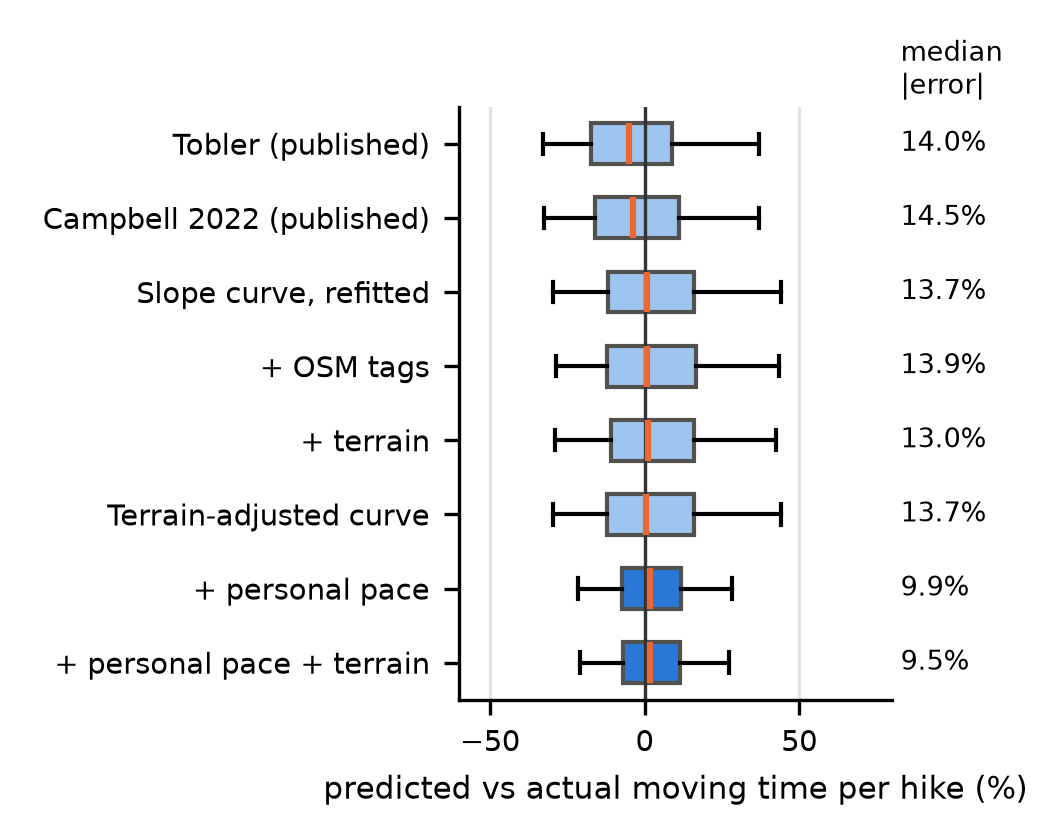
\includegraphics[width=\textwidth]{fig_hike_time}
\column{0.4\textwidth}
\small Moving time per hike, 1,354 hikes in held-out regions (median
error):
\begin{itemize}\setlength\itemsep{4pt}
\item slope curve 13.6\%
\item + terrain 13.0\%
\item + the hiker's own pace (first km) 10.0\%
\item + own pace + terrain \textbf{9.6\%}; about half of hikes within
  $\pm$10\%
\end{itemize}
\end{columns}
\end{frame}

\begin{frame}{Questions}
\begin{enumerate}\setlength\itemsep{6pt}
\item \textbf{Paper framing}: lead with ``terrain from remote sensing
  transfers to new regions; map tags don't'', with Tobler, Campbell and
  STRIDE as baselines. Agree?
\item \textbf{Embeddings}: present AlphaEarth as ``helps locally, transfers
  less''? Try another embedding?
\item \textbf{Lidar understory} (STRIDE's 0.85--1.2 m band): $\sim$12 GB for
  the White Mountains alone. 1--3 regions, or skip?
\item \textbf{Data release}: a de-identified copy is ready; license (ODbL)
  and lab policy?
\item \textbf{Cluster account}: \texttt{engr-class-any} or the lab's?
\item \textbf{Sparse GPS traces} read up to 11\% slow (how we measure).
  Fix in a T1 v2, use only traces logged every $\le$10 s for absolute
  speeds, or report it?
\item \textbf{Figures}: the draft is at 5 pages with 6 figures. Which 3--4
  to keep?
\end{enumerate}
\vspace{6pt}
\small Next: paper draft (skeleton with table and figures exists; full
draft by $\sim$27 Nov; deadline 11 Jan).
\end{frame}

\end{document}
